% Software Frontend (HTML/CSS/JS; Vue.js)
% Zuständig: Arthur

\chapter{Software - Frontend}
\initials{AB}
\label{sec:software_frontend}
Das Frontend wurde als Webanwendung realisiert,
welche die vom Server gesammelten Daten visualisiert.
%
Dazu zählen z.B. die Daten vom LiDAR-Sensor,
vom Beschleunigungssensor
und die Geschwindigkeit der Roboter,
welche mithilfe der Encoder ausgelesen wird.
%
Um die Aktivitäten der Roboter mitverfolgen zu können,
ohne vor Ort anwesend sein zu müssen,
werden auch die Livestreams von Kameras,
welche auf den Robotern angebracht sind,
angezeigt.
\\\\
Das Frontend wird mithilfe von Vue.js programmiert.
%
Vue.js ist ein JavaScript-Framework zur Webentwicklung
und bietet verschiedene Möglichkeiten,
Webseiten zu programmieren.
%
Bei Vue.js kann man zwischen der ``Options'' oder
der neueren ``Composition'' API unterscheiden.
%
Die Composition API ist etwas flexibler in der Anwendung,
während die Options API eine klar definierte Struktur verfolgt.
%
Letztlich ist es dem Entwickler überlassen,
je nach seinen Präferenzen zu wählen.
%
Wir verwenden für unsere Anwendung die Composition API,
da diese etwas intuitiver ist
und ``normalem'' JavaScript etwas näher kommt. 
%
Der große Vorteil des Vue.js Frameworks ist,
dass man einzelne Komponenten einer Website
als sogenannte SFC\footnote{Single-File Components}s definiert.
%
Wie der Name schon impliziert ist in diesem SFC alles enthalten,
was diese Komponente braucht: HTML, CSS und Type-/JavaScript.
%
Dadurch wird der Code schön strukturiert und klar aufgeteilt.
%
Des Weiteren können Vue-Komponenten auch
in anderen Komponenten wiederverwendet werden,
was eine schöne Abstrahierung ermöglicht.

\section{Webseite}
\initials{AB}
\label{subsec:frontend_Webseite}
Nach der Einführung des Frontendes in Kapitel \ref{sec:software_frontend} folgt eine detaillierte
Beschreibung der Webseite sowie ihrer Funktionen. 
%
Wie bereits erwähnt, dient die Webseite der Veranschaulichung 
und bearbeitung der Daten die vom Server empfangen werden. 
%
Diese Daten werden als rohe Binärwerte empfangen und dann im Code der Webseite,
genauer im Modul ``websockets.vue'' deserialisiert werden. 
Das Deserialisieren stellt sicher, dass die übertragenen Informationen in einer für den Benutzer 
verständlichen und brauchbaren Form bereitgestellt werden. 
%
Das Hauptziel der Webseite ist es, die empfangenenen Daten des Servers in brauchbare Werte umzuwandeln. 
Diese umgewandelten Daten werden dann für weitere Berechnungen verwendet sodass eine sinvolle grafische Darstellung
erstellt werden kann.
%
Die grafische Darstellung der verschiedenen unterteilten Sensorwerte ermöglicht dem Nutzer Muster sowie 
Zusammenhänge zu erkennen. 
%
Die grafische Darstellung soll für jeden Sensor unterschiedlich erfolgen. So können potentielle Schwierigkeiten 
der Roboter grafisch analysiert werden. Dies kann beim interpretieren helfen und zukünftige Fehler vorbeugen. 
%
Nicht nur sollen die Daten angezeigt werden, dass wichtigste ist es die empfangen Daten 
in Echtzeit anzeigen zu lassen, sodass stets die neusten und aktuellsten Informationen präsentiert werden können.
%
Die Webseite ist so aufgebaut, dass sofern ein weiterer Sensor implementiert werden sollte, 
der Code mit leichtigkeid erweitert werden kann und es zu keinen weiteren Schwierigkeiten kommen kann.  
\\ \\
Zur Veranschaulichung der Systemarchitektur wurde ein Flussdiagramm erstellt, 
das die interaktionen zwischen den einzelnen Komponenten genau darstellt.
Das Flussdiagramm dient der Analyse der Kommunikationswege innerhalb des Systems und
zeigt perfekt, welche Komponente als Sender bzw. als Empfänger agiert. 
%
\begin{figure}[H]
  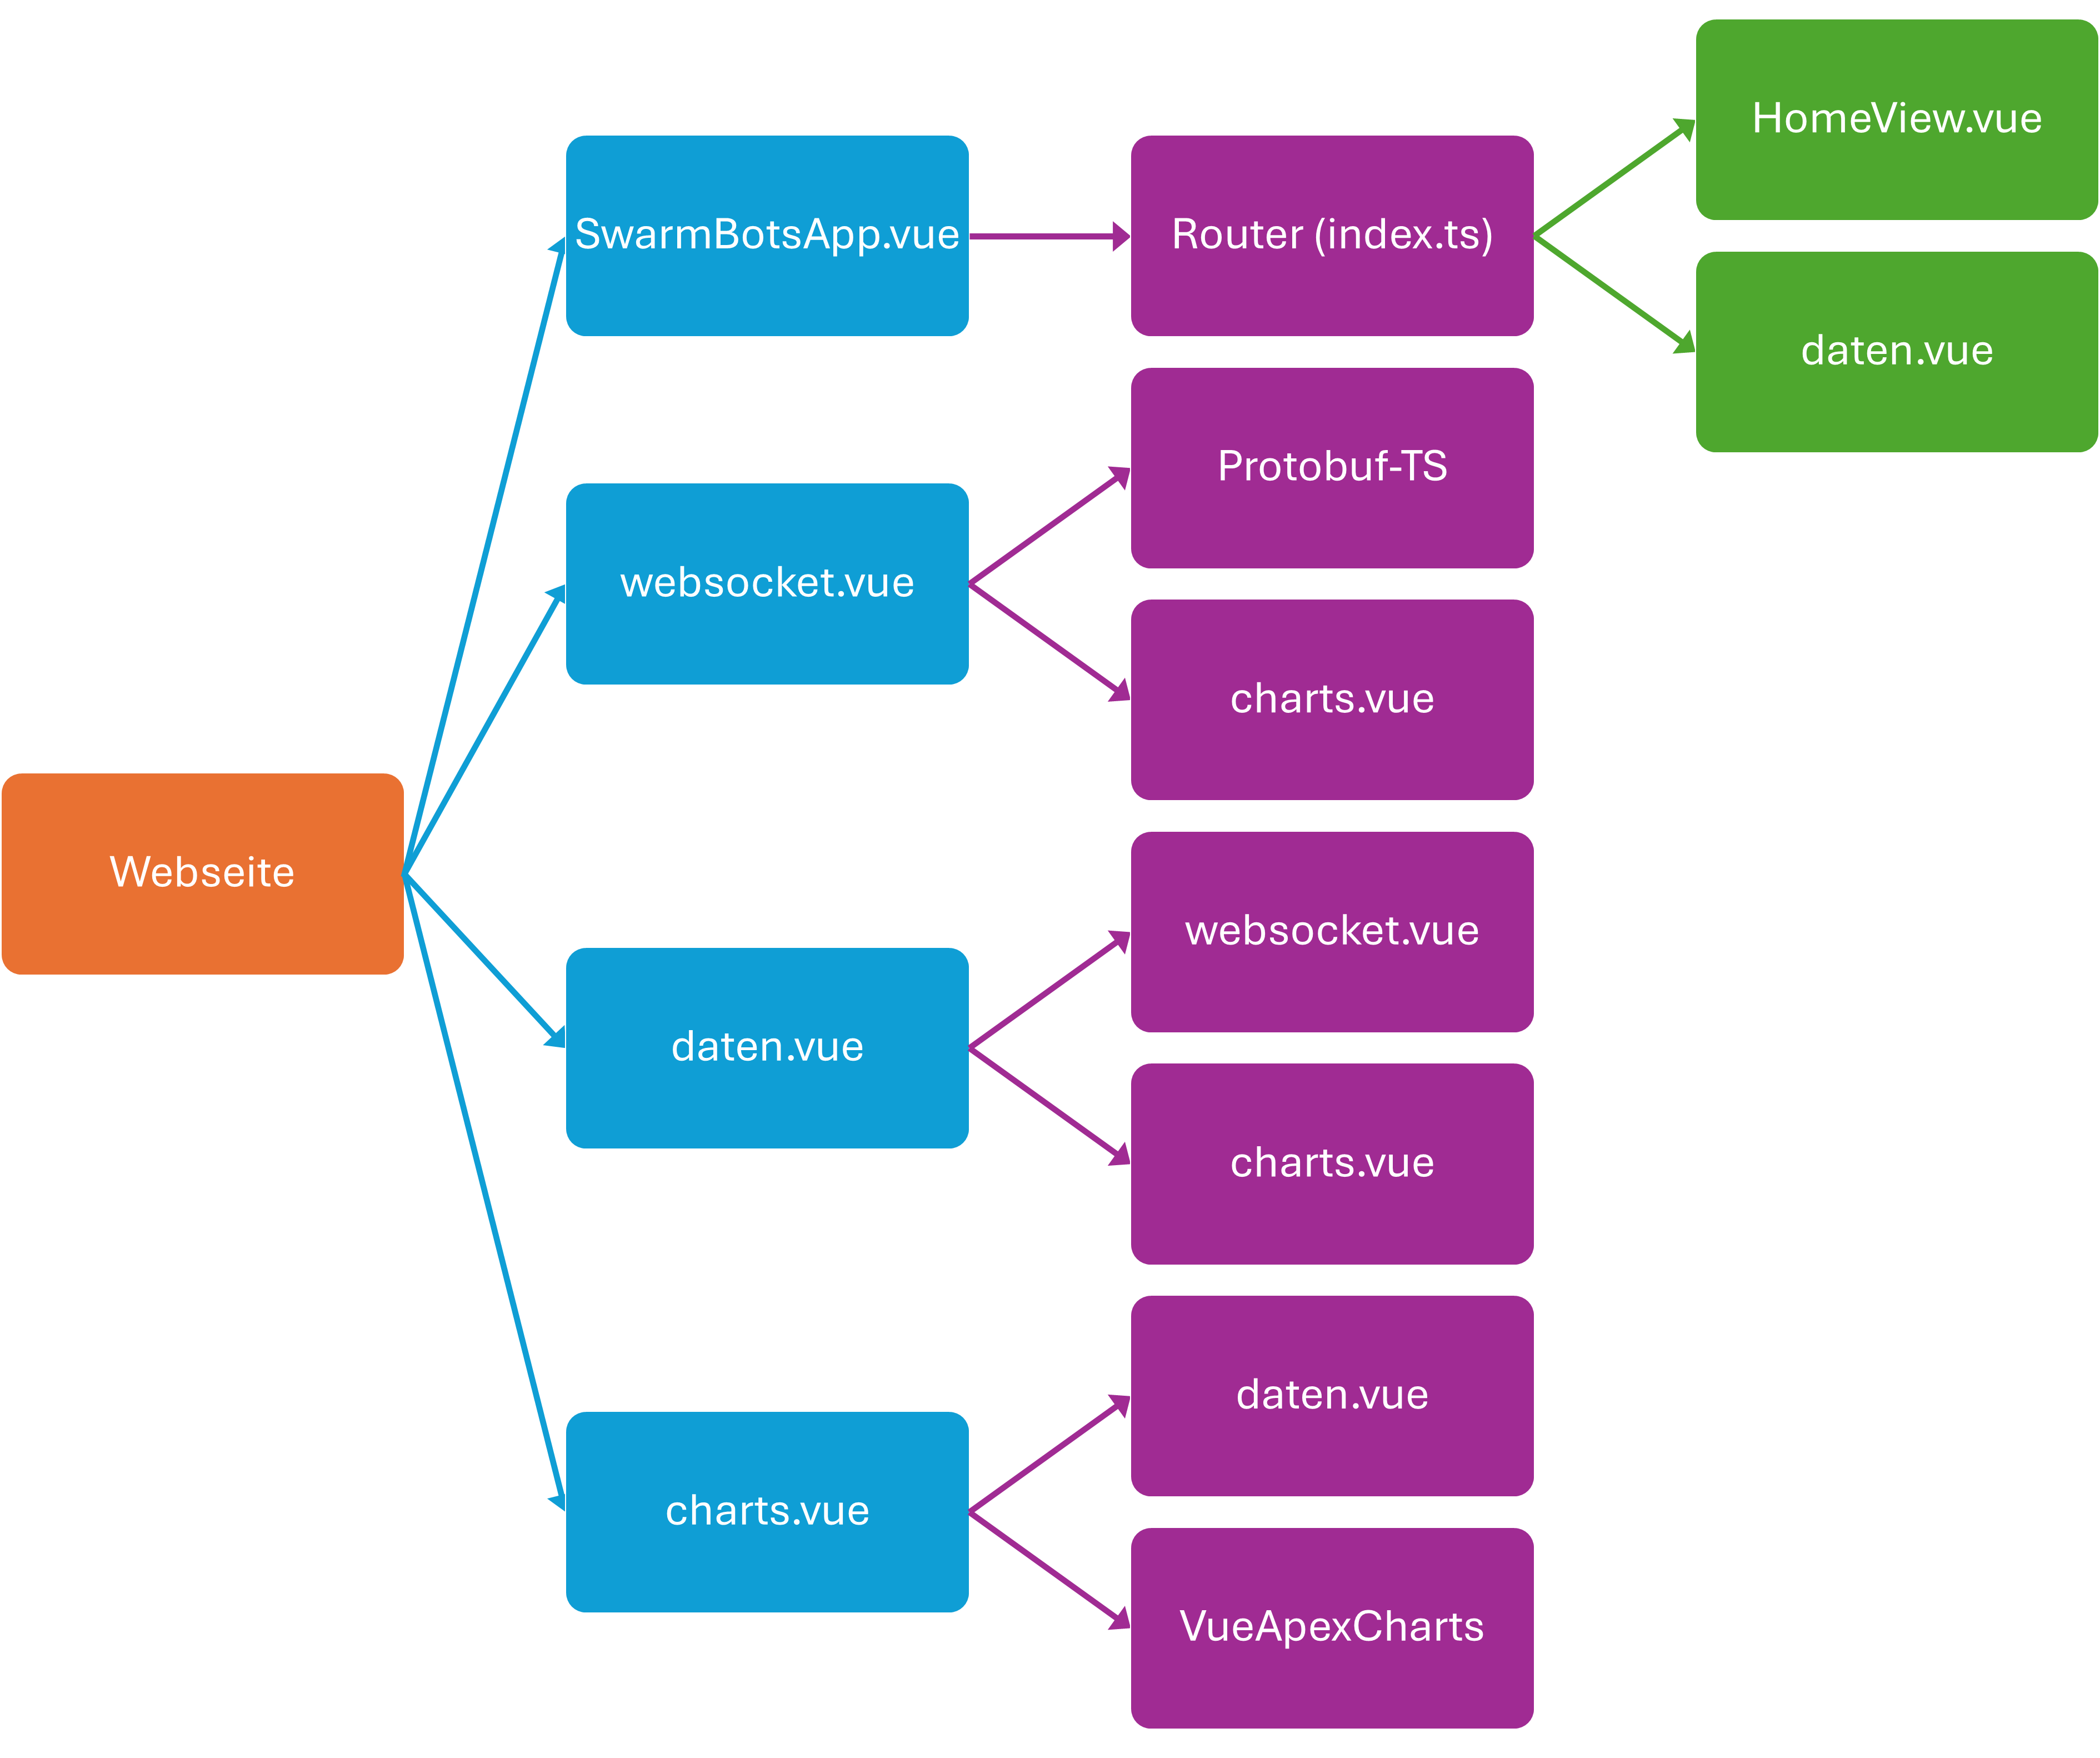
\includegraphics[width=\textwidth, center]{img/Webseite_FD.png}
  \caption{Webseite - Flussdiagramm}
  \label{fig:Webseite_Flowchart}
\end{figure}

\subsection{Webseite - Startseite}
\initials{AB}
\label{subsubsec:Webseite_Startseite}

\begin{figure}[H]
  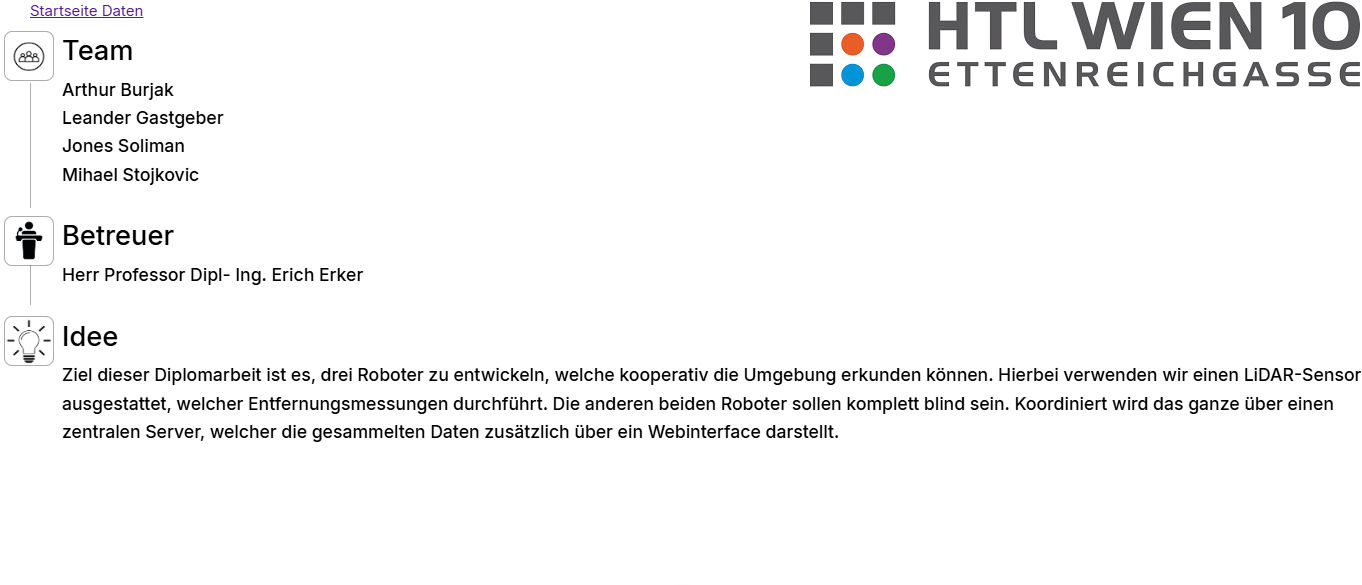
\includegraphics[width=\textwidth, center]{img/Webseite_Startseite.png}
  \caption{Webseite - Startseite}
  \label{fig:Webseite_Startseite}
\end{figure}

Zu sehen ist die fertige Startseite der Diplomarbeitsgruppe ``SwarmBots''. 
Die Umsetzung der Benutzeroberfläche erfolgt unter Verwendung von CSS im Hauptmodul ``SwarmBotsApp.vue''.
%
Das Hauptmodul ``SwarmBotsApp.vue'' beinhaltete ursprünglich alle Komponenten, wurde jedoch im Laufe des Projektes
auf den derzeitigen Stand aufgeteilt um einen bessern Überblick zu gewährleisten.
%
Das Hauptmodul dient derzeitig nur für die Formatierung der Startseite, die auslesung, verarbeitung 
sowie Veranschaulichung der Sensordaten werden in den einzelnen Komponenten erledigt. 
%
Die Startseite bietet dem Nutzer einen übersichtlichen Einstieg in das Projekt. Sie stellt die Mitglieder des Teams
sowie den zuständigen Betreuer vor und vermittelt einen ersten Eindruck der Diplomarbeit. \\
% 
\\
Die Startseite erfüllt zwei wichtige Punkte: Der erste, sie soll dem Nutzer als Informationsquelle der 
Diplomarbeit dienen sowie über ihrer Gruppenmitglieder und ihrem Betreuer. 
Der zweite wesentliche Punkt der Startseite ist es die Navigationslinks anzuzeigen um zu den 
gesammelten Sensordaten zu kommen. 

\subsection{Webseite - Daten}
\initials{AB}
\label{subsubsec:Webseite_Daten}

\begin{figure}[H]
  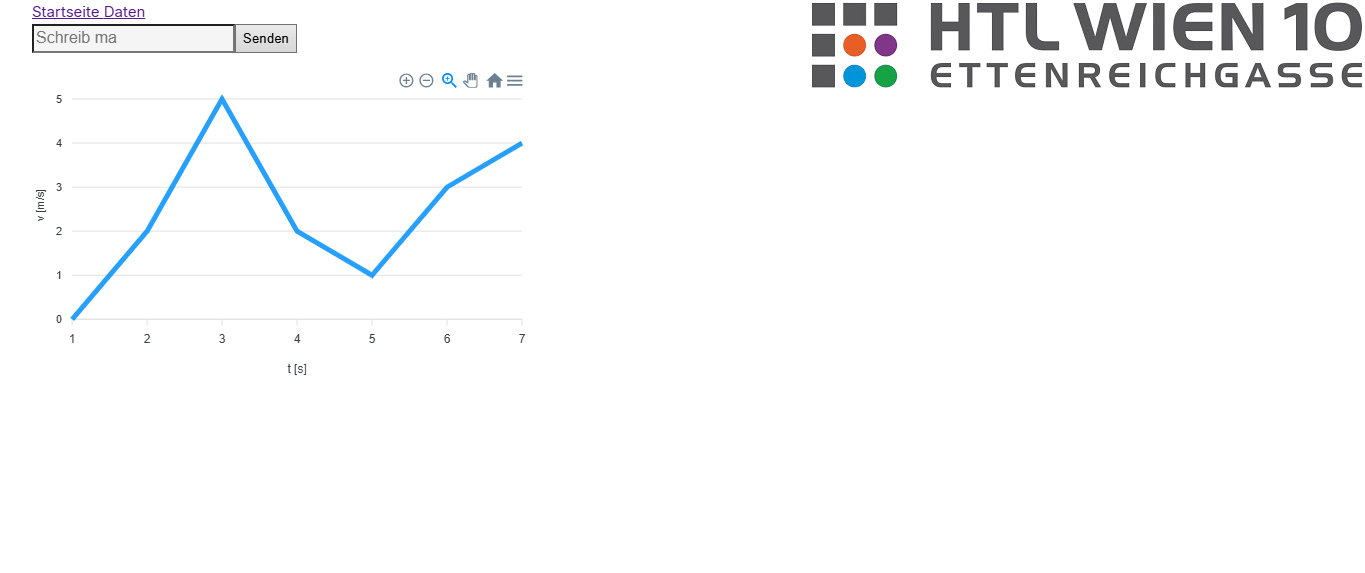
\includegraphics[width=\textwidth, center]{img/Webseite_Daten.png}
  \caption{Webseite - Daten}
  \label{fig:Webseite_Daten}
\end{figure}

Dieser Teil der Webseite ist für die Darstellung sämtlicher emfpangener Daten verantwortlich.
Die empfangenen Daten der Sensoren werden grafisch visualisiert und dem Nutzer in beschrifteten Diagrammen dargestellt. 
%
Zusätzlich neben der vielen gesammelten Sensordaten, wurde ein Websocket integriert, 
der eine zweiseitge Kommunikation mit dem Server ermöglicht. 
%
Die bereitstehende Websocket verbindung dient zur schriftlichen Kommunikation mit dem Server bei etwaigen problemen.
%
Dieser Abschnitt der Webseite ist Aufgrund der Datenvisualisierung der wichtigste im Bereich des Frontends.

\section{LiDAR-Karte}
\initials{AB}
\label{subsec:frontend_lidar_map}
Die LiDAR-Karte wird im Frontend mithilfe von Vue.js generiert und in stetig aktualisert. 
Die Karte dient der Darstellung von Hindernissen in der Umgebung und zeigt Objekte wie Wände, 
Säulen oder auch Personen in Form von Punktwolken an. 
%
Der LiDAR-Sensor bietet leider keine detaillierte Darstellung der Punktwolke, 
weshalb das Herauslesen unterschiedlicher Hindernisse in manchen Fällen zu Schwierigkeiten führt. 
%
Die Karte soll außerdem zwischen einem Hinderniss sowie den Robotern ``Tamerlan'' und ``Bambi'' 
unterscheiden und diese Hervorheben. 
%
Jedoch sollen nicht nur Hindernisse grafisch dargestellt werden, 
sondern auch die aktuellen Positionen der SwarmBots.
%
Das auslesen der Position der SwarmBots ermgöglicht dem Nutzer mögliche Probleme zu erkennen, 
z.B. wenn die SwarmBots probleme beim erkennen einiger Objekte haben sollten.  

\begin{figure}[H]
    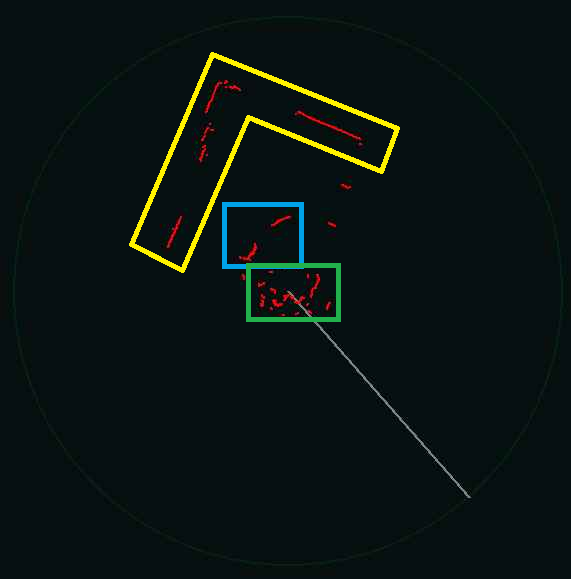
\includegraphics[width=0.7\textwidth, center]{img/LiDARMessungZeichnung_alt.png}
    \caption{LiDAR-Messung}
    \label{fig:LiDAR-Messung}
\end{figure}

Das Bild zeigt die generierte Punktwolke des LiDAR-Sensors.
%
Die Punktwolke zeigt ideal die Funktionsweise des LiDARs
und ist leicht zu interpretieren.
%
Die unterschiedlichen Laserimpulse,
welche gesendet werden,
reflektieren an der Oberfläche und werden gemessen.
\\\\
Zur einfacheren Interpretation des Beispiels
wurden von Herrn Burjak Bereiche eingezeichnet:
%
Der grüne Bereich zeigt Objekte,
welche unmittelbar vor dem LiDAR standen.
%
In dem Fall waren es Büromaterialien wie etwa Kugelschreiber, Hefte, etc.
%
Blau markiert ist eine Person (links),
die ungefähr in 2.5 m Entfernung vom Sensor
neben einem Sessel (rechts) steht.
%
Im gelbem ``L'' kann man die Wände bzw. Bücherregale erkennen,
welche den Testraum abgegrenzt haben.
Die beiden großen Lücken im gelbem Bereich wurden
durch die Hindernisse im blauem Bereich verursacht,
an denen der Laser bereits schon frühzeitig abgeprallt ist.
%
Die beiden nicht markierten Punkte-``Cluster'' stellen Dachstützen dar.

\section{Anzeigen der Sensordaten}
\initials{AB}
\label{subsec:frontend_sensors}
Die Sensordaten werden alle auf dem Frontend dargestellt und stetig aktualisiert.
%
Jeder Tumbller-Roboter ist ab Werk mit Beschleunigungssensoren und Drehgebern ausgerüstet,
welche wir gleich für unsere Zwecke wiederverwendet haben.
%
Als Modifikationen haben wir jedem Roboter ein Kompass-Modul
und Guide zusätzlich noch den LiDAR installiert.
%
Der LiDAR erstellt eine Karte in Form einer Punktwolke,
um eventuelle Hindernisse erkennen zu können.
%
Für mehr Informationen zum LiDAR-Sensor siehe Abschnitt \ref{subsec:ueberblick_lidar} oder \ref{subsec:frontend_lidar_map}.

\begin{figure}[H]
    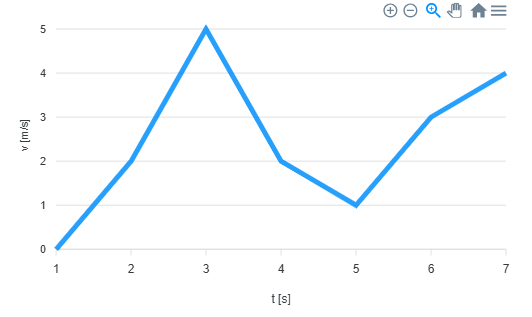
\includegraphics[width=0.8\textwidth, center]{img/encoder_chart.png}
    \caption{Diagramm der Encoderdaten}
    \label{fig:Encoderdaten}
\end{figure}

Die Werte der Beschleunigungssensoren werden,
im Graphen abhängig von der Zeit angezeigt, 
um die aktuellen Werte mit der Vergangenheit vergleichen zu können.

\section{Fernüberwachung per Kamera}
\initials{AB}
\label{subsec:frontend_cam_stream}
Auf allen drei Robotern befinden sich fest montierte
\texttt{ESP32-CAM}-Kameramodule zur Überwachung,
welche dem Frontend via MJPEG ein Live-Bild bereitstellen.
%
Die Kameras dienen vor allem der Überwachung der Roboter und sollen der Gruppe nur helfen,
mögliche Probleme (z.B. Stiegen) rasch zu identifizieren,
um die Sicherheit der Roboter zu gewährleisten.
%
Eingriffe erfolgen nur falls die Roboter nicht selbstständig erfolgreich die Gefahrensituation vermeiden.
%
Sollte ein Fehler bei der autonomen Steuerung von einem der Roboter aufgetreten sein,
helfen uns die Kameras zusätzlich bei der manuellen Fernsteuerung.
%
So können wir mithilfe der Fernsteuerung (Siehe Abschnitt \ref{subsec:frontend_control}) probieren,
die Roboter z.B. aus einer Gefahrenzone zu entfernen.

\section{Fernsteuerung}
\initials{AB}
\label{subsec:frontend_control}
Das Konzept der Fernsteuerung wurde aus den Prototypen der Projektwoche aus dem Jahr 2023/2024 übernommen.
%
Diese hatten eine Fernsteuerungsfunktion per Playstation 4 Controller. Einfachkeitshalber wurden die Roboter über 
den Laptop mittels Playstation 4-Controller angesteuert. 
%
Das größte Problem der Playstation 4-Controller besteht darin, dass sie jedes mal ihre MAC-Adresse ändern sofern
man sie über die Roboter verbindet.  
%
Die Fernsteuerungsfunktion sollte aber nur zu Testzwecken dienen um die Roboter 
vor potentiellen Gefahrensituation zu Retten. 

\section{Frontend - Code}
\initials{AB}
\label{subsec:frontend_Code}
In diesem Kapitel wird sich hauptsächlich auf die Beschreibung der verschiedenen Module des
Frontend-Codes konzentriert. Die Struktur und Funktionalität werden mit der \texttt{``4+1 architectural view model''} beschrieben.
%
Diese Methode wird häufig bei Softwarelastigen Projekten eingesetzt, um komplexe Systeme aus unterschiedlichen
Perspektiven verständlich darzustellen.
Das 4+1 architectural view model kombiniert die fünf Sichten:
\begin{itemize}
  \item Logische Sichte
  \item Entwicklungssicht
  \item Prozesssicht
  \item Physische Sicht
  \item Szenarien
\end{itemize} 
Der Einsatz des Modells hilft bei der Beschreibung Frontend-Codes. 
Dabei wird der Code nicht nur auf seine technische Umsetzung beschreiben,
sondern auch auf seine Funktion im Gesamtsystem 
sowie seiner Abhängigkeit und interaktion mit anderen Komponenten des Projektes.

\subsection{Protobufs generieren - TypeScript}
\initials{AB}
\label{subsec:proto_gen_TS}
Bevor die Struktur sowie das Verhalten der Codes im Detail erläutert werden können,
müssen zunächst die Protobuf-Dateien generiert werden. 
%
Die Webseite verwendet die generierten Protobuf-Definitionen in TypeScript, 
um die benötigten Daten korrekt interpretieren und verarbeiten zu können.
%
Nach der grundlegenden Einführung in Abschnitt \ref{subsec:ueberblick_protobufs}, 
in dem die Gründe für den Einsatz von Protocol Buffers genannt werden, 
beschreibt dieses Kapitel den Prozess der Generierung dieser Dateien.
%
Zu Beginn der Diplomarbeit wurden die Protobuf-Datein manuell generiert. 
Da sich dieser Vorgang jedoch als sehr zeitaufwändig erwies,
wurde der Prozess im laufe der Diplomarbeit durch ein automatisiertes Skript ersetzt.
%
Dieses Skript wird automatisch ausgeführt, sboald die Webseite gebaut oer gestartet wird.
Es hat dabei stets die höchste Priorität, wodurch sichergestellt ist, 
dass der Code stets mit den aktuellsten generierten TypeScript-Dateien arbeitet.
%
Der zentrale Teil des Generierungsprozesses sieht wie folgt aus:
\begin{lstlisting}[language=JavaScript, gobble=4]
  {
    exec("npx protoc --proto_path=../proto --ts_out=./src/lib/ ../proto/*.proto", (error, stdout, stderr) => {
            if (error)
              console.error('\n'+error.message)
            if (stderr)
              console.error('\n'+stderr)
            if (stdout)
              console.log('\n'+stdout)
        })
        console.log("Compiled protobufs!")
  }
\end{lstlisting}
Die Funktion führt den Befehl zur Generierung der Protobuf-Dateien sofort aus und speichert die erzeugten Dateien
im Verzeichnis ``lib''. 
Dieses Verzeichnis dient als Zielordner für alle generierten Protobuf-Dateien für die Webseite.

\subsection{SwarmBotsApp.vue}
\initials{AB}
\label{subsec:frontend_SwarmBotsApp.vue}
Der Code ``SwarmBotsApp.vue'' beschreibt eine einfache Navigations- und Anzeige-Komponente
für die Webseite und nutzt Vue-Router um diese Links verwenden zu können.  
%
Der Code erstellt mithilfe von Vue-Router zwei Navigationslinks zur Verfügung,
der eine Link führt zur Startseite und der andere zum Link Daten. 
%
Basierend auf welchen Link man drückt, ändert sich der Inhalt der Webseite.
%
Zusätzlich wird in der Komponente statisch das HTLW10 Logo eingeblendet was als Layout für alle weiteren 
Links dienen soll. 
%
Als Hilfestellung wurde ein Flussdiagramm erstellt, 
welches die genauen Abläufe des Codes zur Erstellung der Navigationslinks wiederspiegelt.
\begin{figure}[H]
  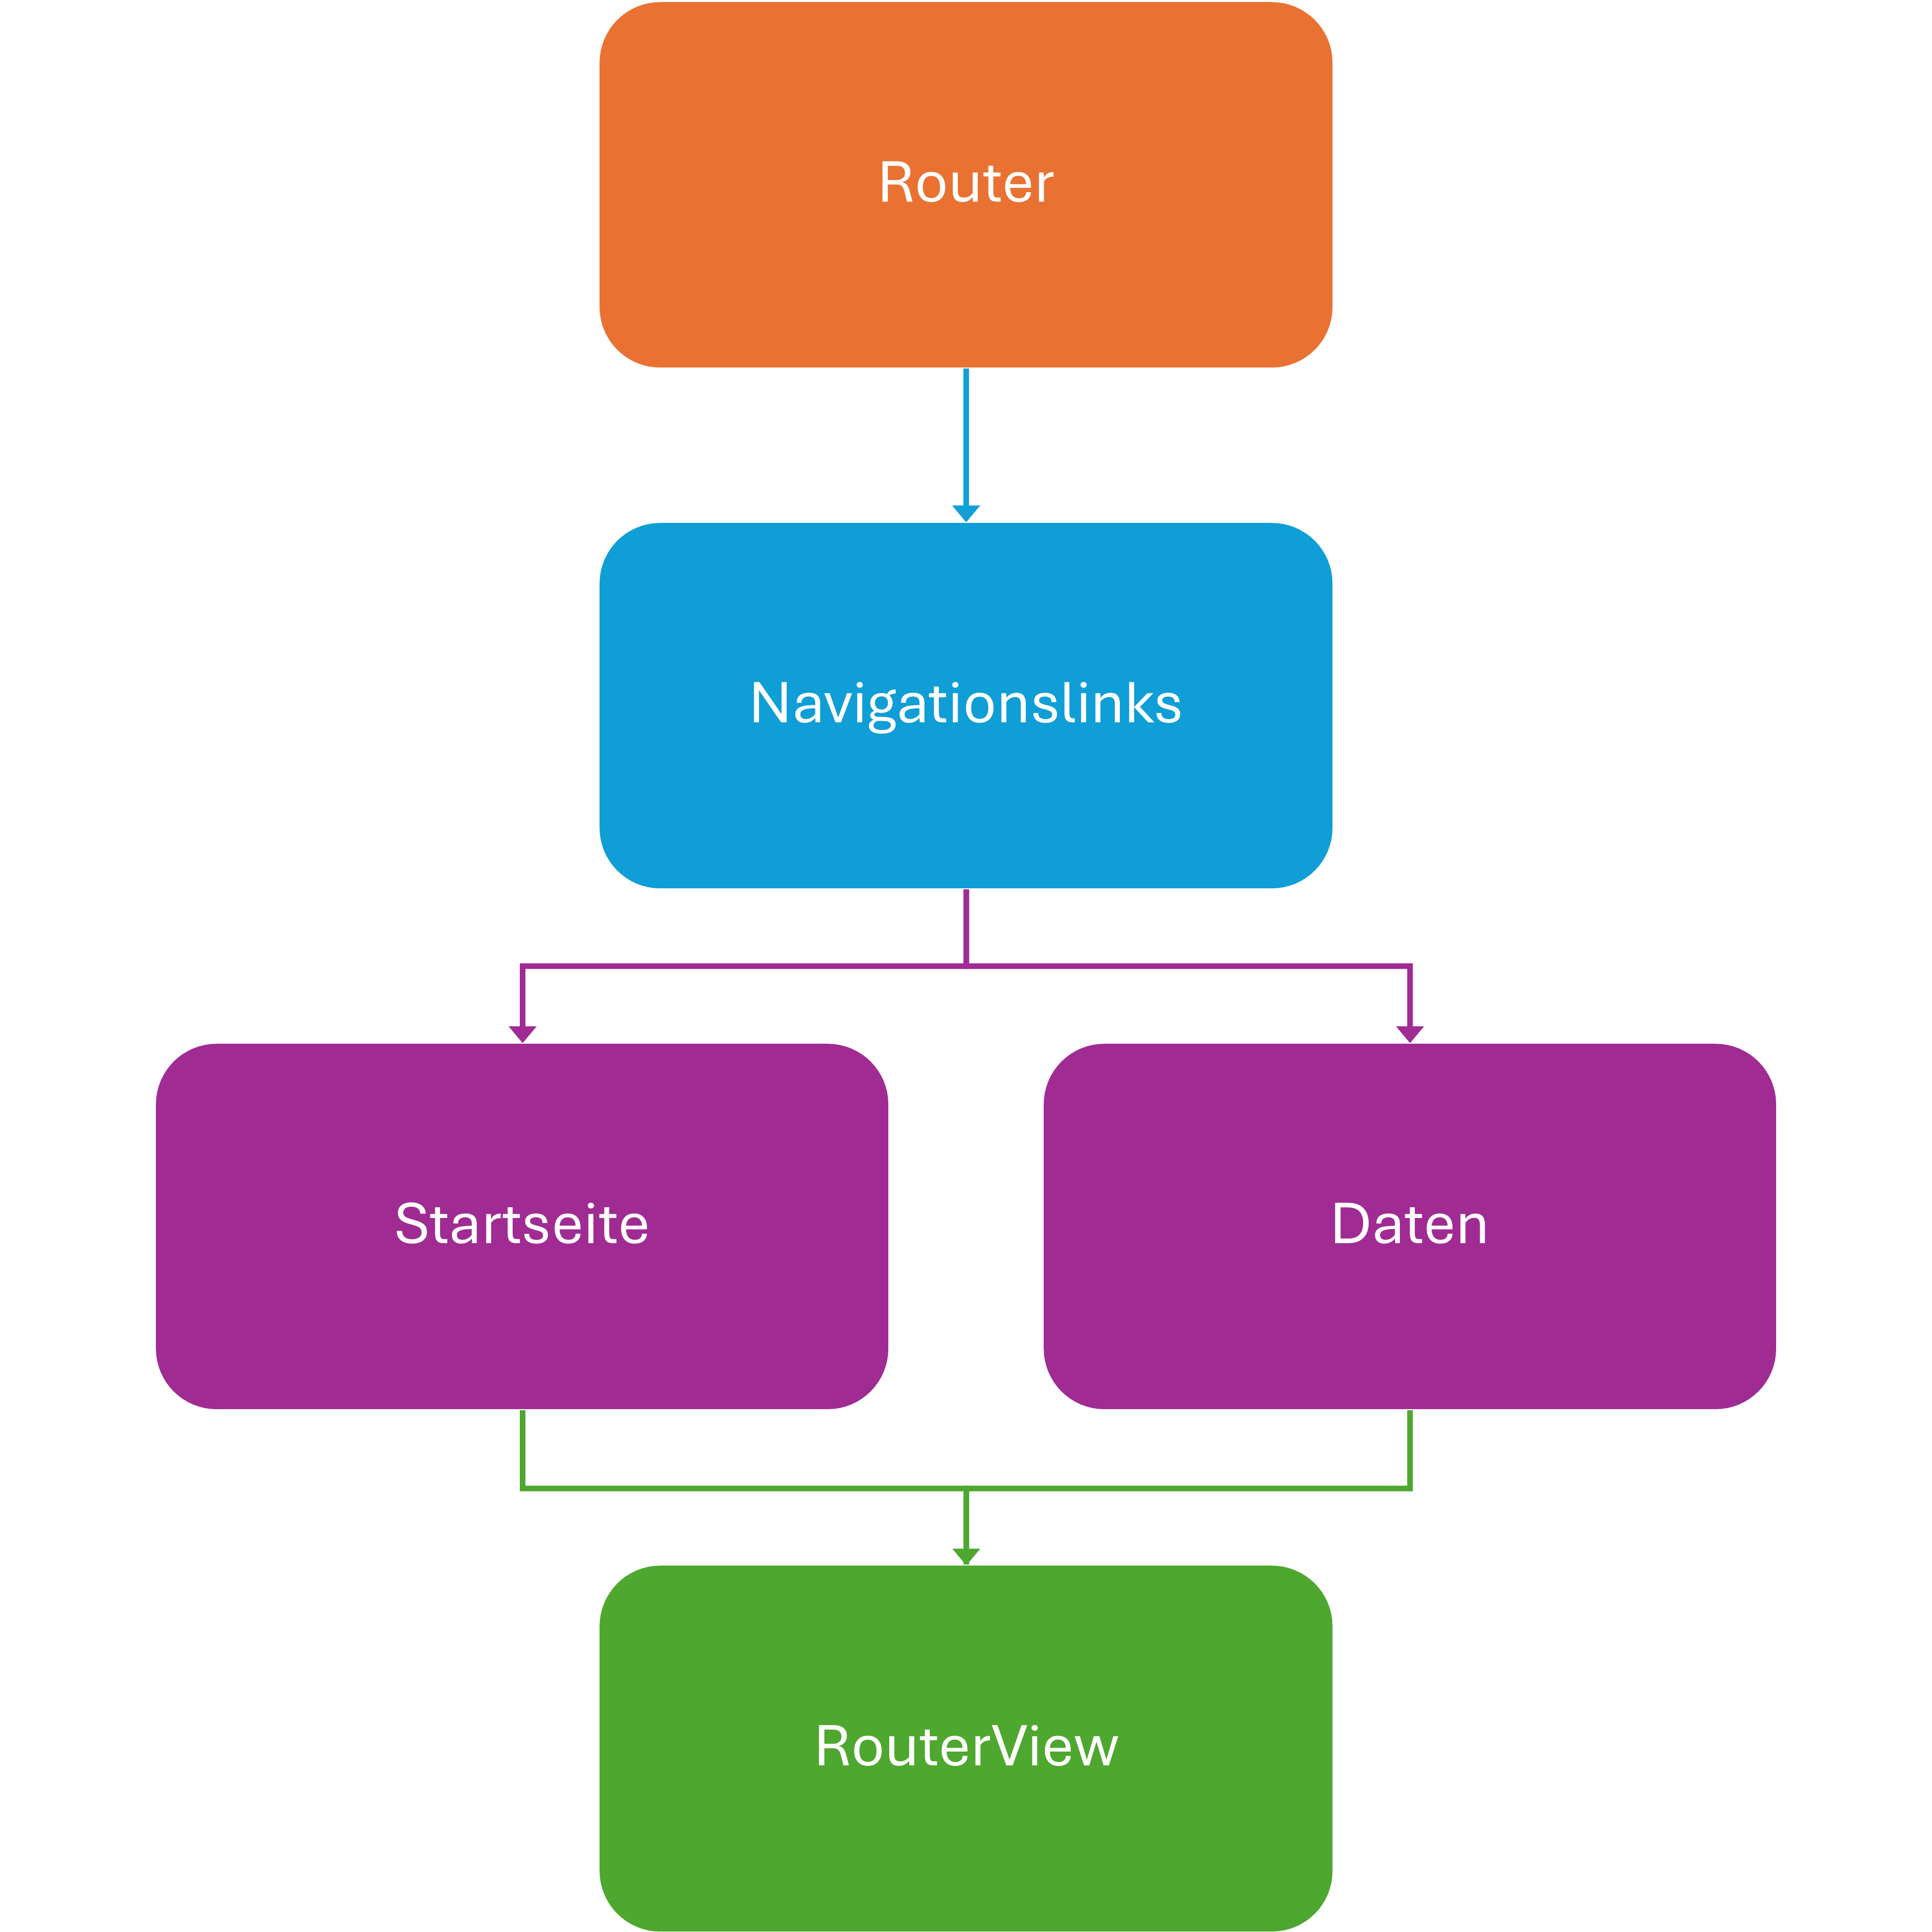
\includegraphics[width=0.8\textwidth, center]{img/SwarmBotsApp_FD.png}
  \caption{SwarmBotsApp.vue - Flussdiagramm}
  \label{fig:SwarmBotsApp_Flowchart}
\end{figure}

  \begin{enumerate}
    \item \texttt{Logische Sicht:} \\
    Die Komponente ``SwarmBotsApp.vue'' bildet das Grundgerüst der Webseite.
    %
    Sie stellt die Navigationsfunktion zur Verfügung und dient als Layout für die Webseite.
    %
    Über die beiden Navigationspunkte kann der Benutzer per Knopfdruck zwischen der Startseite
    und der Datenseite wechseln.
    %
    Zusätzlich wird ein statisches Logo der HTLW10 angezeigt, das Teil der globalen Layouts ist.
    \item \texttt{Entwicklungssicht:} \\
    Es wird Vue3 mit TypeScript verwendet. 
    %
    Die Navigation basiert auf dem ``Vue-Router'' (für mehr Infos siehe Abschnitt \ref{subsec:frontend_VueRouter}).
    %
    Die Struktur der Komponente ist einfach gehalten und folgt den Richtlinien der SFC. 
    \item \texttt{Prozesssicht:} \\
    Zur Laufzeit der Webseite ermöglicht die Komponente eine Navigation zwischen den Ferstern Webseite und Daten.
    %
    Die Routerlinks-Elemente lösen bei einem Knopfdruck eine Routenänderung aus, 
    woraufhin der entsprechende Inhalt geladen wird, zu dem der Link führt.
    %
    Die Anzeige des Logos der HTLW10 sowie das Layout sind unversell. 
    \item \texttt{Physische Sicht:} \\
    Die Komponente wird im Browser, als Bestandteil einer Vue-basierten SPA\footnote{Single Page Application} ausgeführt
    \item \texttt{Szenarien:} \\
      \begin{itemize}
        \renewcommand{\labelitemi}{$\Rightarrow$}
      \item Der Nutzer öffnet die Webseite.
      \item Der Nutzer kann zwischen verschiedenen Seiten mithilfe der Navigaitonsleiste wechseln.
      \end{itemize}
  \end{enumerate}

\subsection{Vue Router}
\initials{AB}
\label{subsec:frontend_VueRouter}
Vue Router ist die offizielle Routing-Bibliothek für Vue.js. Sie ermöglicht es, 
SPA mit mehreren Seiten bzw. Ansichten zu erstellen. 
%
Das alles funktioniert ohne, dass das die Seite neu geladen werden muss. 
%
Vue Router sorgt dafür, dass eine Webseite mithilfe von Navigationslinks 
zu unterschiedliche Komponenten führt. 
Dabei hat jede Komponente ihre eigene URL, z.B. /Daten, /Kontakte, usw.

Der zentrale Teil des Codes schaut so aus:
\begin{lstlisting}[language=JavaScript, gobble=4]
  {
    <div class="Router">
      <RouterLink to="/">Startseite </RouterLink>
      <RouterLink to="/daten">Daten </RouterLink>
      <br>
      <RouterView></RouterView>
    </div>
  }
\end{lstlisting}

\subsection{websocket.vue}
\initials{AB}
\label{subsec:frontend_websocket.vue}

Bevor die genauer Erklärung bezüglich des websockets.vue Codes kommt,
folgt ein Flussdiagramm, das erstmals die Funktionen und einzelnen Schritte
des Codes beschreibt.
%
Das Flussdiagramm zeigt perfekt die einzelnen Schritte, 
die der Code durcharbeitet um die Geschwindigkeit der Encoder herauszufinden.
Über das Flussdiagramm ist ebenso zu sehen, 
dass der Websocket die Werte für die Diagramme aktualisert. 
%

\begin{figure}[H]
  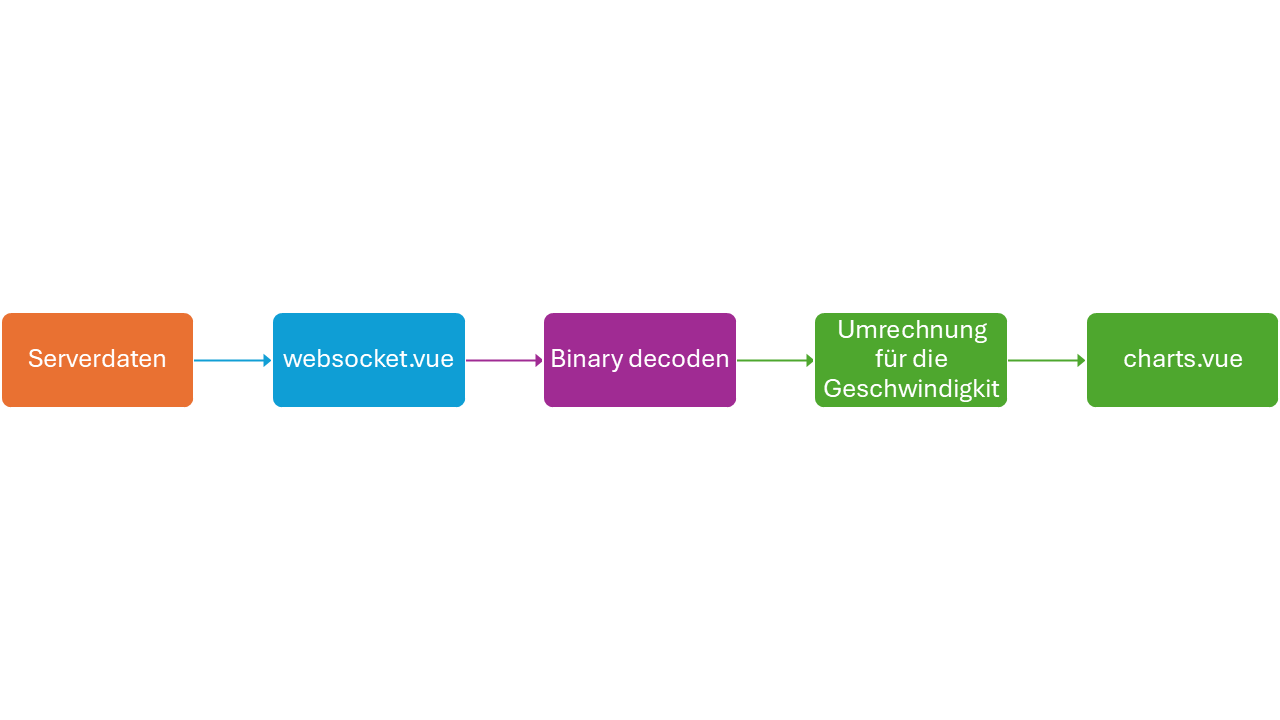
\includegraphics[width=\textwidth, height=14.8cm, center]{img/Websocket_FD.png}
  \caption{websocket.vue - Flussdiagramm}
  \label{fig:websocket_Flowchart}
\end{figure}

\begin{enumerate}
  \item \texttt{Logische Sicht:} \\
  In der logischen Sicht des 4+1 architectural view models ist das Websocket eine esenzielle Komponente.
  %
  Diese Komponente übernimmt die Kommunikation mit dem Server und verarbeitet die empfangenen Daten.
  %
  Die Komponente deserialisiert diese Daten wodurch sie lesbar werden. Nach der Verarbeitung werden die Daten an 
  eine weitere Komponente (charts.vue) gesendet um grafisch dargestellt werden zu können.
  \item \texttt{Entwicklungssicht:} \\
  Aus der Entwicklersicht ist die Komponente ziemlich fortschrittlich.
  %
  Es wird eine aktuelle Version von Vue verwendet (3.5.13), sowie die neuere Composition-API in Kombination mit TypeScript.
  Dadurch das die vielzahl an Komponenten alle aufgeteilt worden sind,
  ist die Fehlersuche sowie die potenzielle Erweiterung des Codes leicht.
  \item \texttt{Prozesssicht:} \\
  Die Kommunikation erfolgt hauptsächlich Eventgesteuert. 
  %
  Beim Eintreffen neuer Daten vom Server, erscheinen sie direkt auf der Grafik, 
  welche dann unter dem Navigationslink ``Daten'' einzusehen sind.
  % 
  Das Empfangen der Daten erfolgt in Echtzeit, so dass die Seite nicht neugeladen werden muss, 
  außerdem werden alte Daten aus der Grafik entfernt und durch neue ersetzt.
  \item \texttt{Physische Sicht:} \\
  Die Webseite welche mittels dem Vue-Framework geschrieben worden ist läuft nur im Browser.
  Die notwendigen Server- oder Websocket Verbindungen werden automatisch beim Start der Webseite ausgeführt.
  \item \texttt{Szenarien:} \\
    \begin{itemize}
      \renewcommand{\labelitemi}{$\Rightarrow$}
    \item Der Nutzer öffnet die Webseite.
    \item Der Nutzer wechselt auf den Reiter ``Daten'' über die Navigationsleiste.
    \item Der Nutzer bekommt einen Einblick auf alle derzeitig erfassten Daten der Roboter grafisch dargestellt.
    \end{itemize}
\end{enumerate}

\subsection{daten.vue}
\initials{AB}
\label{subsec:frontend_daten.vue}
Die Komponente ``daten.vue'' basiert in weiten Teilen auf derselben strukturellen 
und funktionalen Grundlage wie die in Abschnitt \ref{subsec:frontend_websocket.vue} beschrieben 
WebSocket-Komponente. 
%
Beide Komponente ermöglichen eine Interaktion über eine WebSocket-Verbindung.
%
Der große Unterschied liegt jedoch im Anwendungsbereich der Komponente 
``daten.vue'':\\
Während die technischere Fortgeschrittenere Komponente in Kapitel \ref{subsec:frontend_websocket.vue} 
weitaus mehr Funktionen besitzt. 
Ist die Komponente ``daten.vue'' darauf reduziert, 
eine direkte bidirektionale Kommunikation zwischen Nutzer und Server herzustellen.
%
Das bedeutet, dass ``daten.vue'' ausschließlich für den reinen Nachrichtenaustausch über
WebSocket verwendet wird. 
Die Komponente eignet sich somit nur als Nachrichtenaustausch.
%
Zur Veranschaulichung wurde ein Flussdiagramm hinzugefügt:
\begin{figure}[H]
  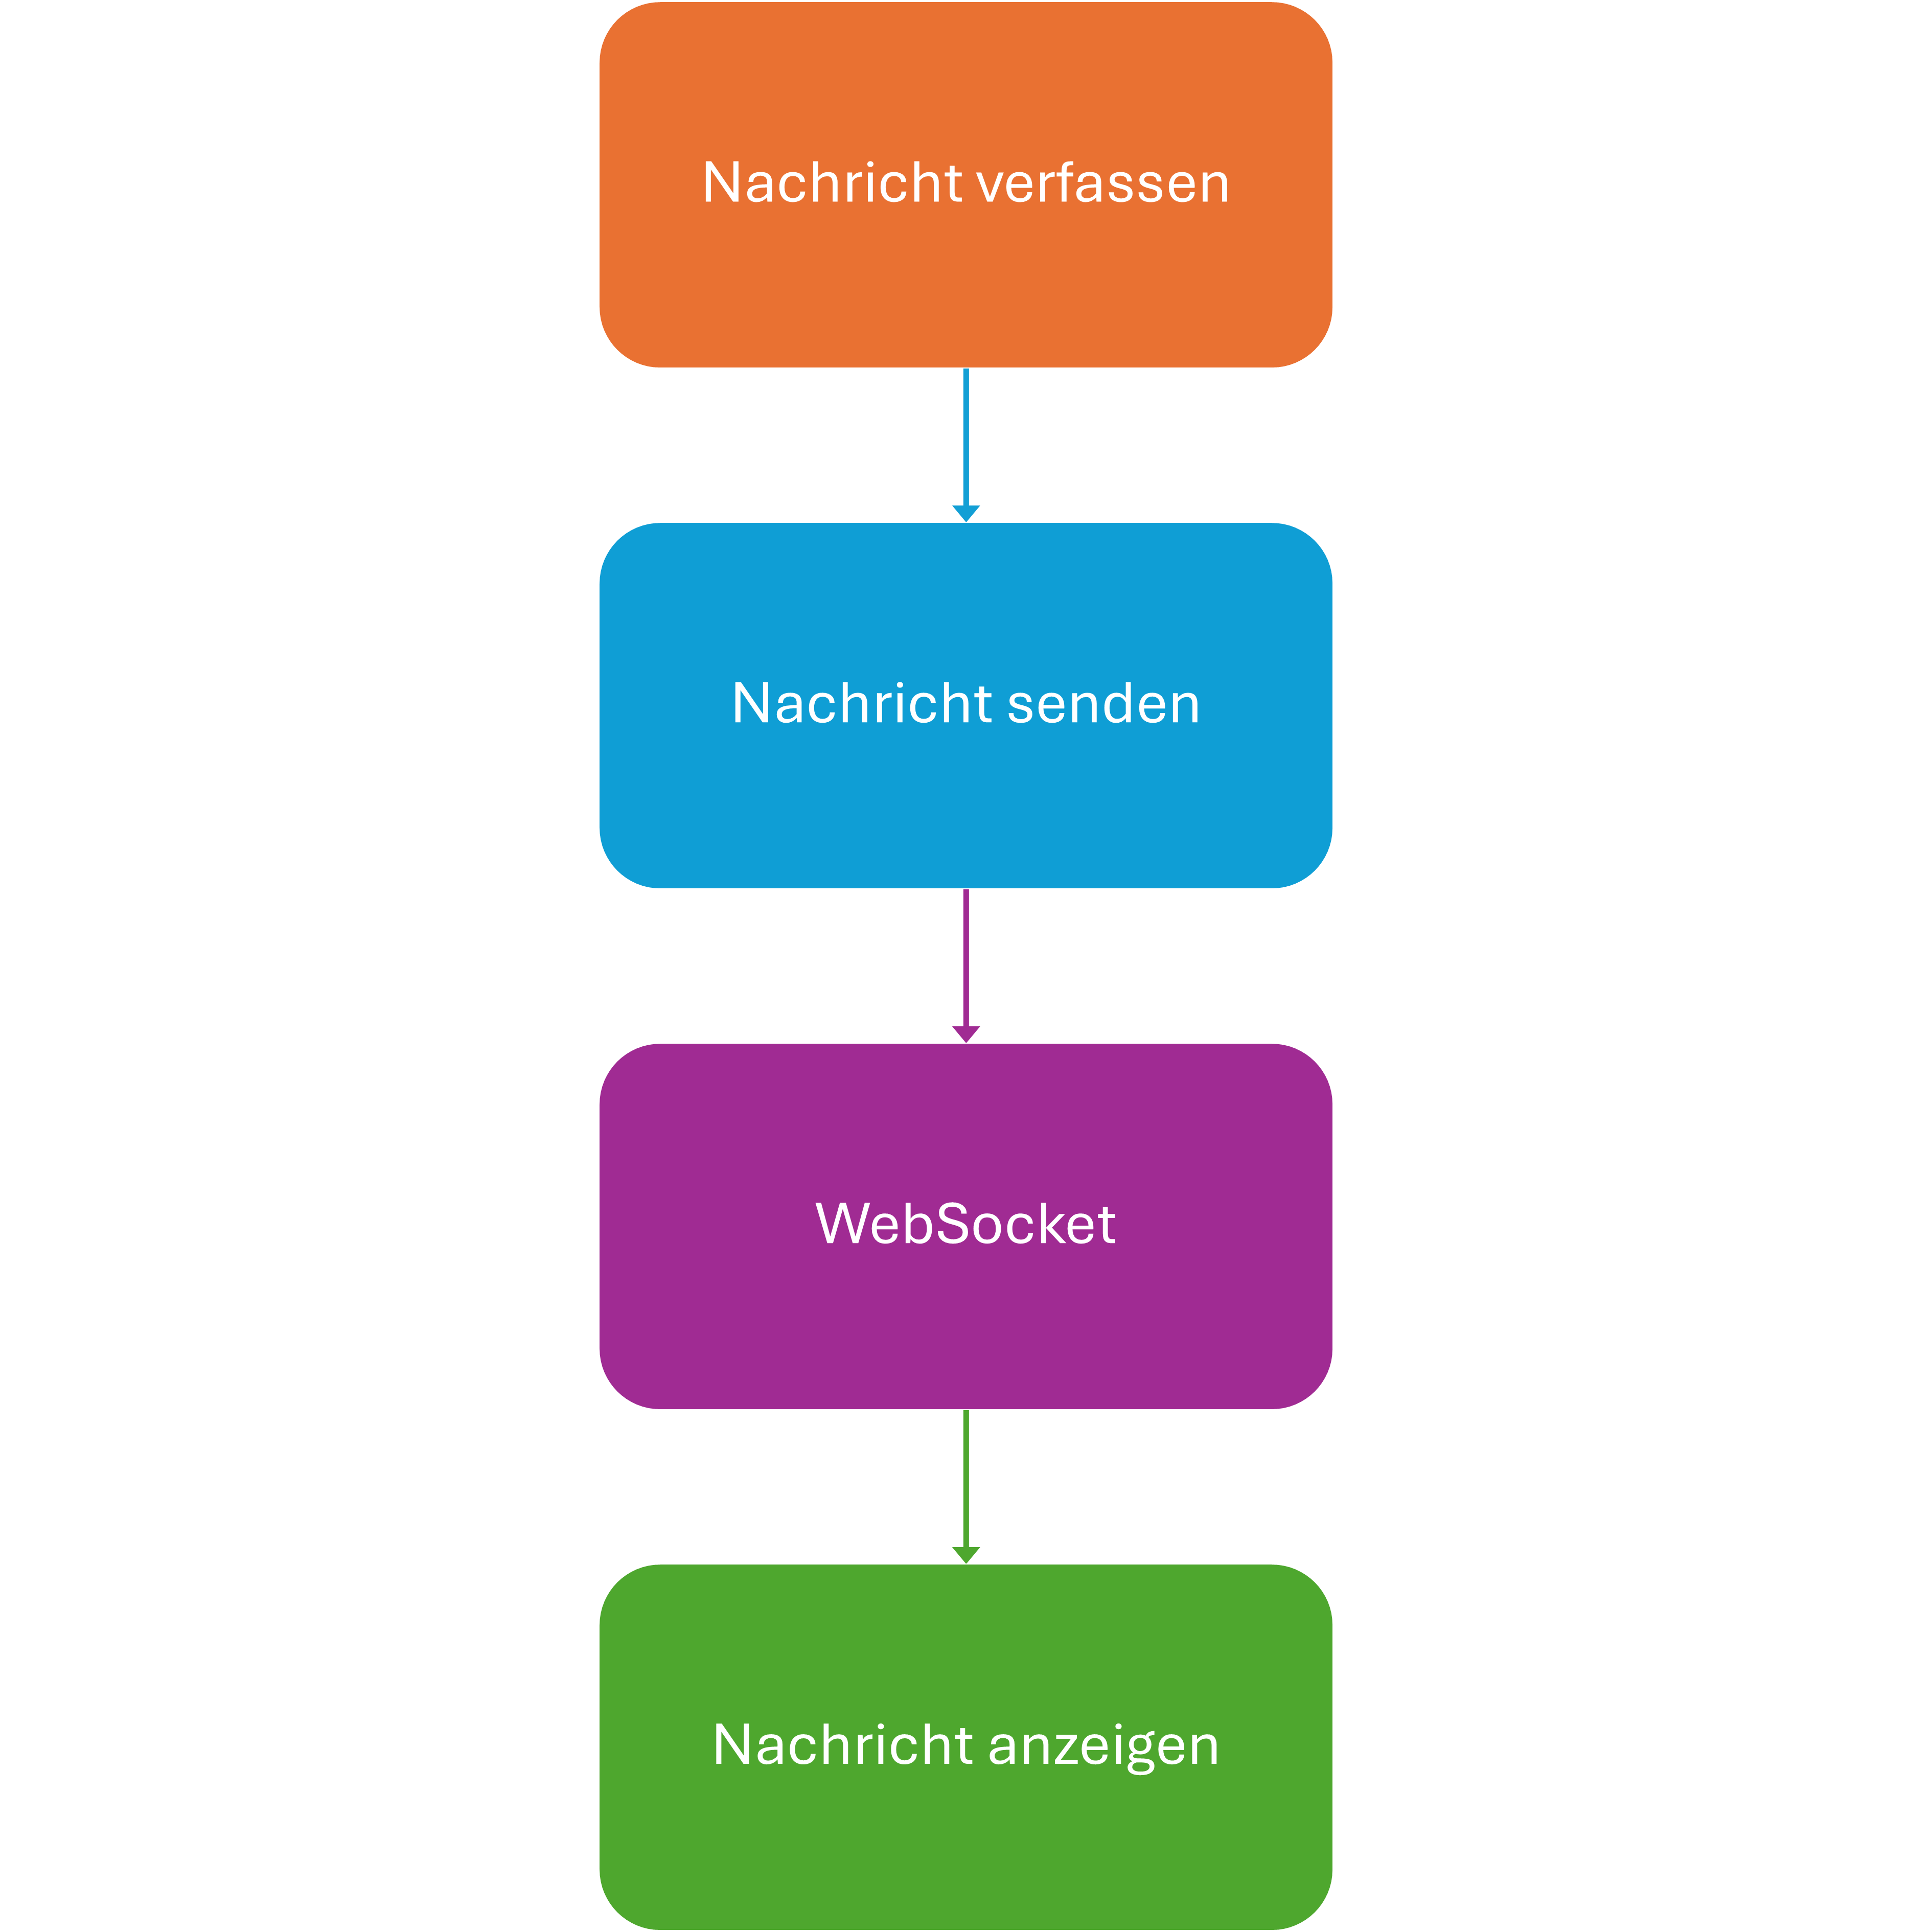
\includegraphics[width=\textwidth, center]{img/Daten_FD.png}
  \caption{daten.vue - Flussdiagramm}
  \label{fig:daten_Flowchart}
\end{figure}

\begin{enumerate}
  \item \texttt{Logische Sicht:} \\
  Diese Komponente stellt eine einfache Benutzeroberfläche für den Nachrichtenaustausch mit einem Server
  über eine WebSocket-Verbindung dar.
  %
  Die Hauptfunktion besteht darin, dass Nutzerinnen und Nutzer eine Nachricht
  in ein Eingabefeld schreiben, diese per Klick auf einen Knopf absenden können und 
  anschließend die gesendete Nachricht um unteren Bereich der Seite angezeigt bekommen.
  %
  Zusätzlich ist eine Diagramm-Komponente eingebunden, 
  welche weitere Daten visualisieren kann.
  %
  Die Logik basiert auf einer reaktiven Datenbindung, die automatisch die Webseite aktualisiert,
  sobald neue Daten hinzugefügt werden sollten.
  \item \texttt{Entwicklungssicht:} \\
  Aus der Entwicklungssicht basiert die Komponente auf Vue3 und verwendet die Composition API
  in Kombination mit TypeScript.
  %
  Die WebSocket-Verbindung ist getrennt von diesem Code geschrieben worden und wird als Modul Importiert.
  Das Diagramm ist ebenfalls ausgelagert und eine seperate Komponente. 
  \item \texttt{Prozesssicht:} \\
  Zur Laufzeit reagiert die Komponente auf Nutzereingaben und führt in Abhängigkeit davon bestimmte
  Aktionen aus. Sobald eine gültige Nachricht eingegeben und gesendet wird, 
  wird diese über die bestehende WebSocket-Verbindung an den Server übermittelt. 
  %
  Gleichzeitig wird die Nachricht auf der Webseite angezeigt.
  %
  Die Komponente kann somit als eine Art leichtgewichtier Client betrachtet werden, 
  der Nachricht sendet, anzeigt und gegebenenfalls weiter Daten über die importierte Diagramm-Komponente visualisiert. 
  \item \texttt{Physische Sicht:} \\
  Die Komponente wird im Browser als Teil einer Vue-Webanwendung ausgeführt. 
  Die Komponente benötigt für die Laufzeit eine funktionierende WebSocket-Verbindung zu einem Server,
  welche Nachrichten empfangen und gegebenenfalls beantworten kann.
  \item \texttt{Szenarien:} \\
    \begin{itemize}
      \renewcommand{\labelitemi}{$\Rightarrow$}
    \item Der Nutzer öffnet die Webseite.
    \item Der Nutzer wechselt auf den Reiter ``Daten'' über die Navigationsleiste.
    \item Der Nutzer gibt eine Nachricht in die Nutzereingabe ein. 
    \end{itemize}
\end{enumerate}

\subsection{charts.vue}
\initials{AB}
\label{subsec:frontend_charts.vue}
Die Komponente ``charts.vue'' sorgt für die Darstellung von Diagrammen,
welche die Messwerte unterschiedlicher Sensoren visuell darstellt.
%
``charts.vue'' nutzt eine externe Bibliotheken (z.B. ApexCharts) zur Diagrammdarstellung.
Dadurch wird eine reaktive Darstellung ermöglicht.
%
Der Code der Komponente ist so aufgebaut, dass mit leichtigkeid weitere Diagramme
mit minimalem Aufwand ergänzt werden können. 
Dabei müssen die weiteren Diagramme nicht statisch sein, 
sondern können ebenso reaktiv aufgebaut sein.
%
Zusammengefasst trägt die ``charts.vue''-Komponente wesentlich zur 
Dateninterpretation bei, indem sie die erfassten Daten,
welche in der WebSocket-Komponente umgewandelt werden, präzise und reaktiv darstellt.

\begin{figure}[H]
  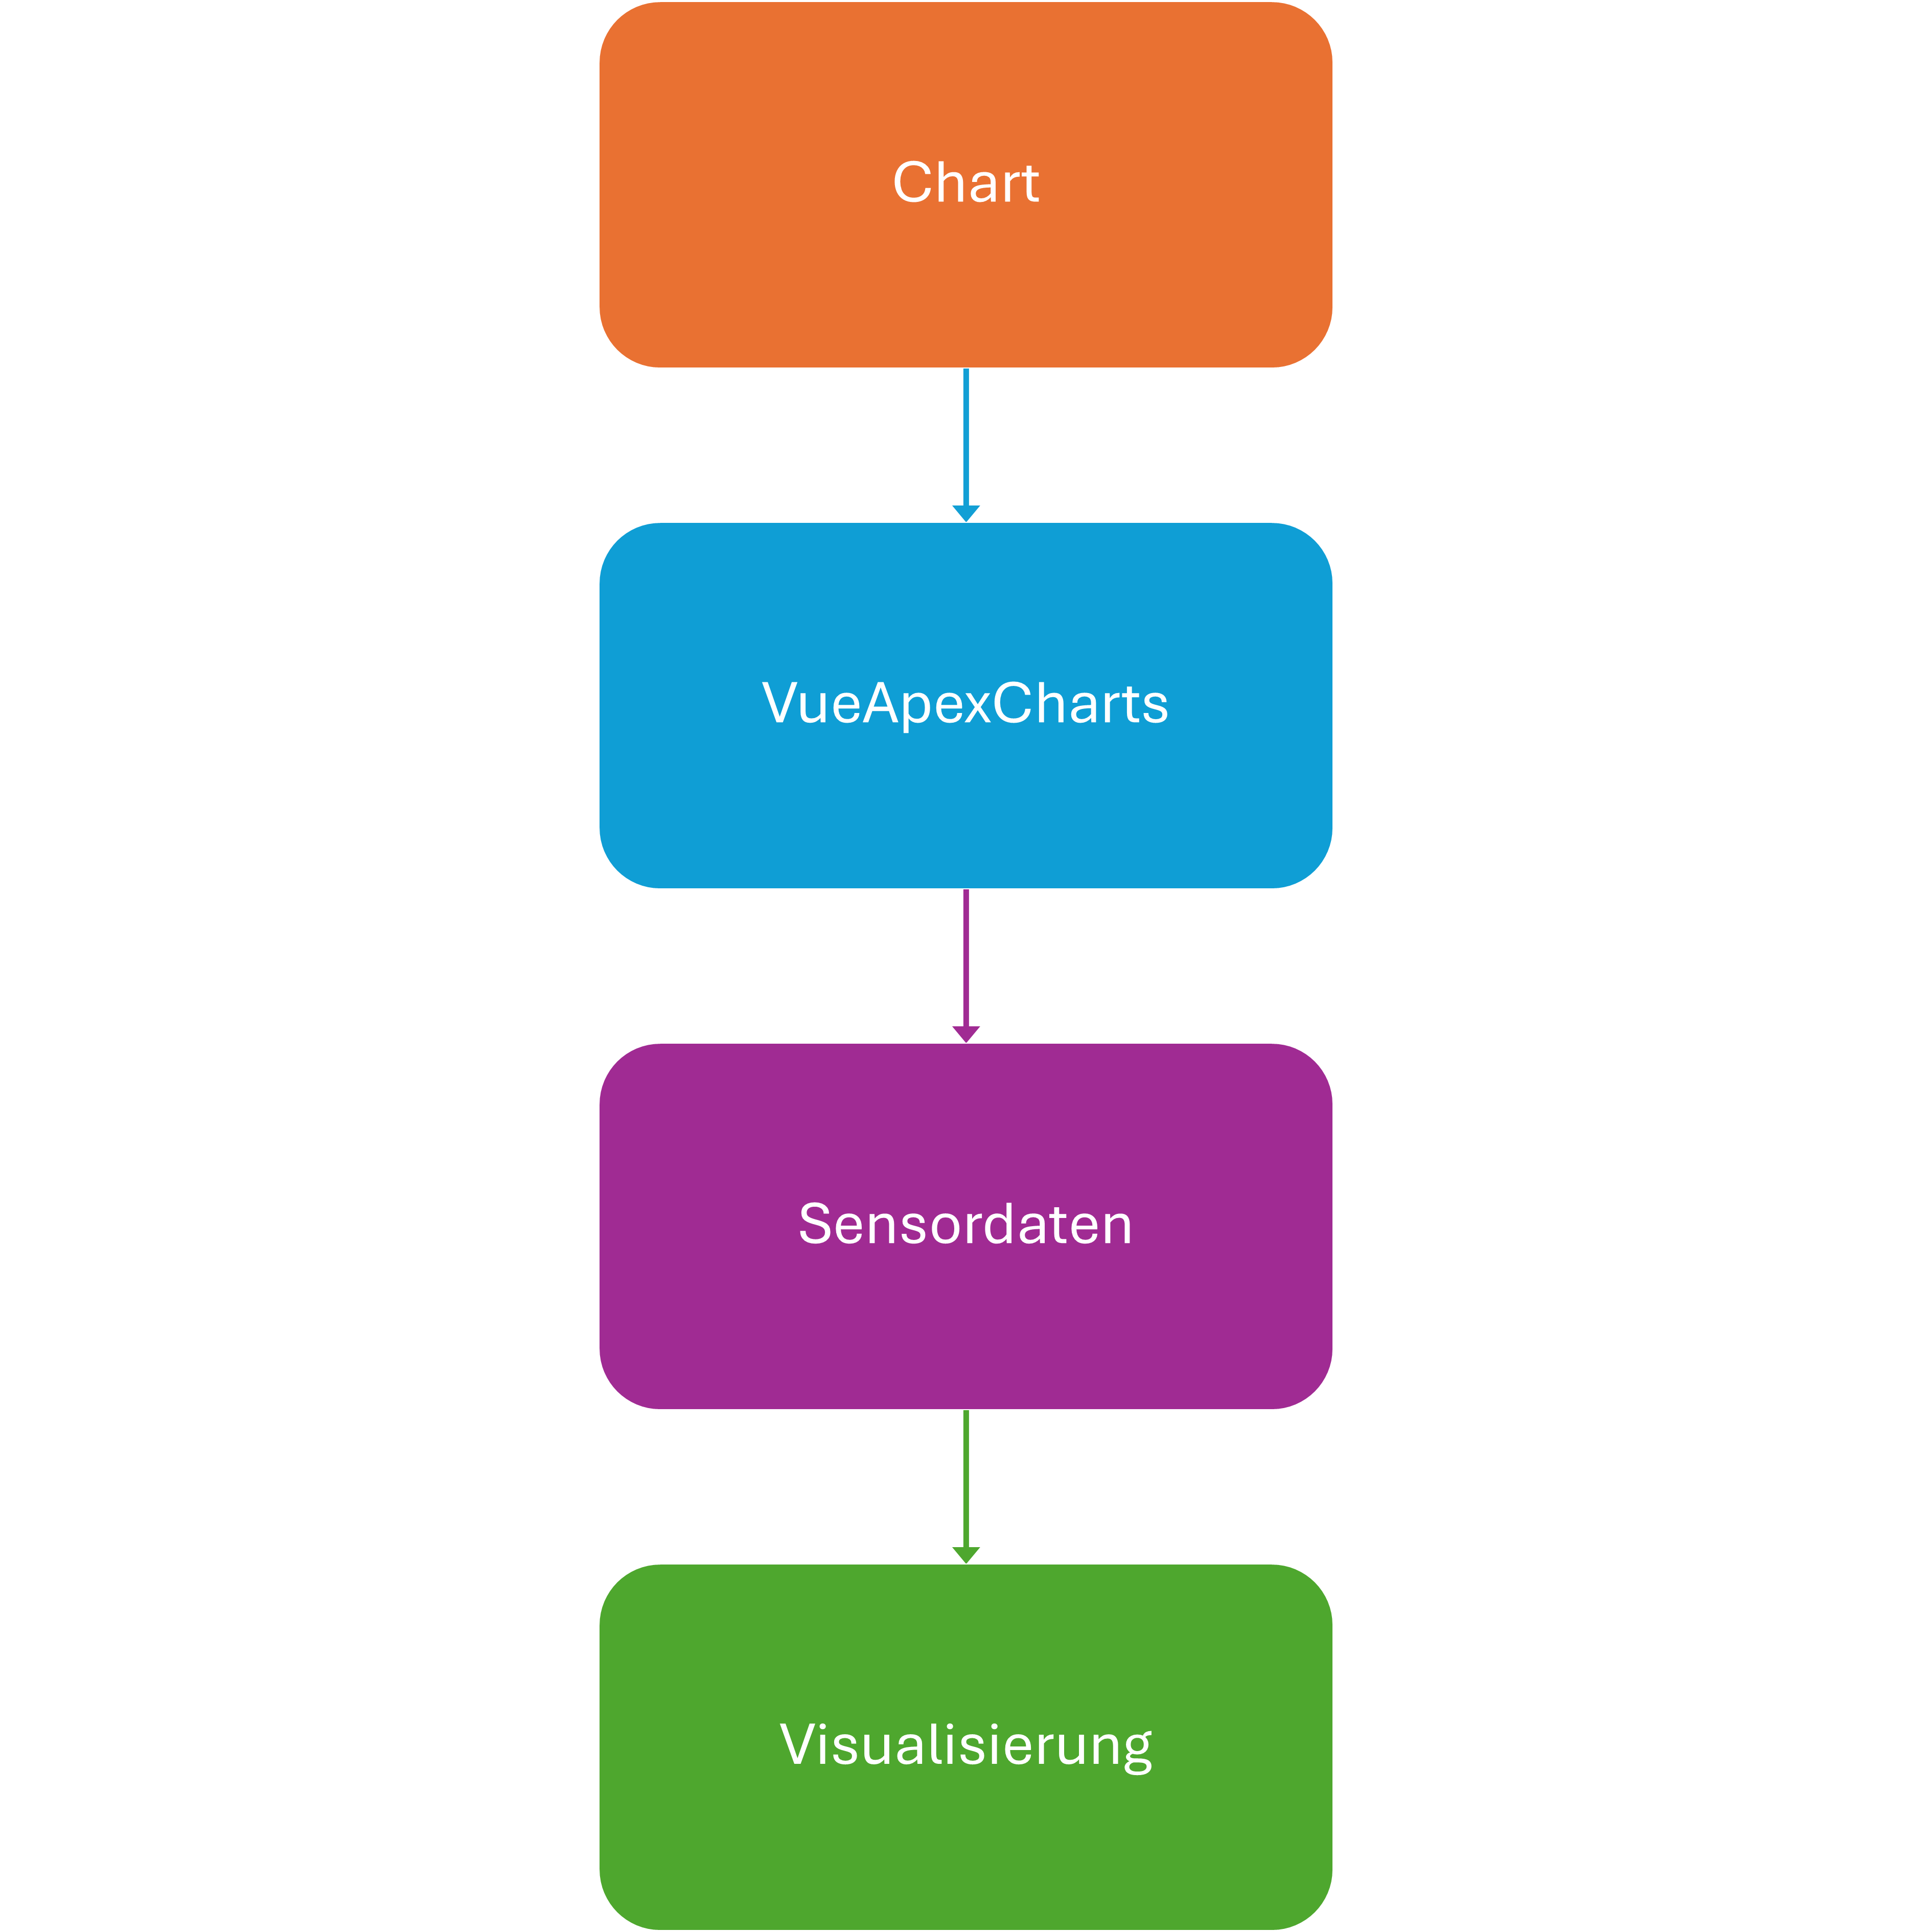
\includegraphics[width=\textwidth, center]{img/Charts_FD.png}
  \caption{charts.vue - Flussdiagramm}
  \label{fig:charts_Flowchart}
\end{figure}

\begin{enumerate}
  \item \texttt{Logische Sicht:} \\
  Diese Komponente dient der Visualisierung der Sensodaten in Form von Diagrammen.
  %
  Die Komponente verwendet die Bibliothek ``ApexCharts''.
  Ziel ist es die empfangenen Sensordaten des Servers zu visualisieren. 
  \item \texttt{Entwicklungssicht:} \\
  Aus der Entwicklungssicht basiert die Komponente auf Vue3 und verwendet die Composition API
  in Kombination mit TypeScript.
  %
  Es wird eine externe Bibliothek importiert um die notwendigen Diagramme zu realisieren.
  Die Komponente ist mit leichtigkeit modulierbar und erweiterbar. 
  \item \texttt{Prozesssicht:} \\
  Zur Laufzeit der Webseite wird die Komponente vom Framework gerendet, 
  wodurch ein interakives Diagramm anhand der empfangenen Daten erzeugt wird.
  %
  Die Diagrammkonfiguration und Datenserie werden bei in reaktiven Datenobjekten gespeichert,
  sodass bei neu erhaltenen Sensordaten, das Diagramm diese automatisch aktualisiert. 
  \item \texttt{Physische Sicht:} \\
  Die Komponente wird im Browser als Teil einer Vue-Webanwendung ausgeführt.
  % 
  Die Abhängigkeit von ApexCharts erfordert, dass die Bibliothek korrekt installiert ist.
  %
  Die empfangenen Sensordaten werden aus anderen Komponenten importiert.
  \item \texttt{Szenarien:} \\
    \begin{itemize}
      \renewcommand{\labelitemi}{$\Rightarrow$}
    \item Der Nutzer öffnet die Webseite.
    \item Der Nutzer wechselt auf den Reiter ``Daten'' über die Navigationsleiste.
    \item Der Nutzer kann über das interaktive Diagramm die Messwerte der Sensordaten auslesen. 
    \end{itemize}
\end{enumerate}

\subsection{Vergleiche}
\initials{AB}
\label{subsec:frontend_Vergleich}

\subsubsection{Warum ApexCharts?}
Beim Frontend wurde sich für die Verwendung von ApexCharts entschieden,
da diese Bibliothek eine Vielzahl an Diagrammtypen unterstützt,
und eine einfache Integration in Vue3 ermöglicht.
%
Neben der vielen unterschiedlichen Diagrammtypen,
bietet die Bibliothek eine Vielzahl an Anpassungsmöglichkeiten,
sowie eine einfache Handhabung.
%
Außerdem bieten die Diagramme von ApexCharts viele Funktionen an, 
welche bei anderen Diagramm-Bibliotheken nicht vorhanden sind, z.B. bei Chart.js.
Diese kleinen Funktionen sind z.B. das ``Tooltip''-Feature,
welches es dem Nutzer ermöglicht, bei Mouseover über einen Punkt, 
die genauen Werte zu sehen oder, das ``Zoom''-Feature, das es dem Nutzer ermöglicht,
einen bestimmten Bereich des Diagramms zu vergrößern.
%
Diese Funktionen sind alle in die Bibliothek integriert und können mit wenigen Zeilen Code aktiviert werden.
Außerdem punktet ApexCharts bei komplexen Diagrammen und datenintensiven Visualisierungen.
% 
\\\\
Bei Chart.js ist dies nicht der Fall,
da diese Funktionen nicht in die Bibliothek integriert sind.
%
Ein Ausschlaggebender Punkt weshalb wir nun ApexCharts verwenden, 
ist die hervoragende Dokumentation der Bibliothek \cite{ApexCharts} 
sowie die Vielzahl an Beispielen, die auf der Webseite zu finden sind.
%
Die Dokumentation und die zahlreichen Beispiele sorgten dafür, 
dass die Gruppe sich für die Bibliothek von ApexCharts entschieden hat.  

\section{Webseitenprobleme}
\initials{AB}
\label{subsec:problem_Webseite}
Im Laufe der Entwicklung der Webseite traten unterschiedliche Probleme auf,
ob nun technischer oder struktureller Natur, 
es wurden alle hier in diesem Kapitel beschrieben.
%
Da die Fehler in Vue3 unter der Verwendung von TypeScript realisiert wurden, 
waren die Fehler nicht immer unmittelbar erkennbar, 
weshalb bei einigen Fehlern die analyse von Mitschülern oder Lehrkräften benötigt wurde.

\subsection{Pfadfindung}
\initials{AB}
\label{subsubsec:problem_Pfadfindung}
Um bei Vue.js Module zu importieren muss die Funktion \texttt{Import from 'PFAD'} verwendet werden.
%
Um die Encoder Daten welche vom Server geschickt werden verarbeiten zu können, 
müssen erstmals die generierten Protobufdateien gefunden werden.
%
\begin{lstlisting}[language=JavaScript,gobble=4]
  {
    import { EncoderData } from  '../lib/encoder_data'
    ...
    const decodedData = EncoderData.fromBinary(binaryData);
    ...
  }
\end{lstlisting}
Es sollte ``EncoderData`` aus der generierten TypeScript-Protobuf Datei gelesen werden und im Modul ``websocket.vue'' verwendet werden.
Dieser Ansatz wie er oben steht, führt jedoch dazu, dass der Pfad nicht gefunden wird. 
%
Nach viel Recherche viel auf, dass nicht nur JavaScript dateien generiert werden müssen, sondern auch TypeScript Dateien.
Sobald die benötigte TypeScript Datei hinzugefügt wurde, verschwand die Fehlermeldung.
%
Nachdem die vorherigen Fehlermeldungen beseitigt worden waren, kam eine neue auf. 
Der Fehler lag, daran, dass die neuen generierten Files das "google-Protobuf" Packet brauchten um zu funktionieren.
% 
\begin{lstlisting}[language=JavaScript,gobble=4]
  {
    import * as pb_1 from "google-protobuf";
    ...
  }
\end{lstlisting}
Dies war leicht zu beheben mit dem Befehl:\\ \texttt{npm install -D @types/google-protobuf} \\ wurden die Packete schnell
heruntergeladen.

\subsection{Variablen einlesung}
\initials{AB}
\label{subsubsec:problem_variablen_einlesen}
Ein hartnäckiges Problem in der Entwicklung des Codes zum Auslesen der Sensordaten, 
stellte das korrekte Einlesen von Variablen aus den generierten TypeScript-Protobuf Dateien dar.
%
Das Generieren der TypeScript-Protobuf Dateien erfolgte wie in Abschnitt \ref{subsec:proto_gen_TS} 
und war kein Problem, was jedoch zu Problemen war das einlesen der notwendigen Variablen, 
welche die Sensordaten beinhalteten. 
% 
\\
Nach der grundlegenden schilderung des Problems, folgen nun die Schritte die zum Problem führten.
%
Der Code wurde geschrieben und die Variablen die in der Protobuf-Datei verarbeiten werden, 
sollten wie folgt eingelesen eingelesen werden.
\begin{lstlisting}[language=JavaScript, gobble=4]
  {
    const pulses = data.pulses;
    const duration = data.duration;
  }
\end{lstlisting}
%
Es wurde mehrere Male überprüft, ob nun wirklich die notwendigen Daten wirklich über die Variable 
``data.pulses'' und ``data.duration'' geschickt werden. 
%
Trotz mehrfacher Überprüfung der Schüler sowie Rückfragen bei Lehrpersonen ob der Code korrekt ist, 
konnte kein Fehler identifiziert werden. 
Laut unseren Überprüfungen waren wir sicher, das die Daten scheinbar korrekt übertragen werden.
%
Nachdem wir als Gruppe nahezu fast jeden erdenklichen Schritt durchgegangen sind, um diesen Fehler zu beheben,
kamen wir als Gruppe auf den Gedanken, die Protobuf-Files mal neu generieren zu lassen, da möglicherweise 
die erstellten Codes Fehler beinhalten konnten. 
%
Daraufhin wurden die Protobuf-Dateien mithilfe des in Abschnitt \ref{subsec:proto_gen_TS} beschriebenen
Befehls erneut generiert.
%
Durch diese neugenerierung wurde die Struktur der TypeScript-Dateien verändert, 
weshalb der Zugriff auf die gewollten Sensordaten nun anders verlief.
%
die neue Änderung sieht wie folgt aus:
\begin{lstlisting}[language=JavaScript, gobble=4]
  {
    const decodedData = EncoderData.fromBinary(binaryData);

    const pulses = decodedData.pulses;
    const duration = decodedData.duration;
    ...
  }
\end{lstlisting}
Der neue Code speichert beide Werte, also data.pulses und data.duration in ``EncoderData''.
EncoderData wird ausgelesen und als ``decodedData'' gespeichert, davon werden die benötigten Werte
dann rausgelesen und weitergeschickt.

\subsection{Diagramm anzeigen}
\initials{AB}
\label{subsubsec:problem_chart_anzeige}
Ein weiteres Problem welches auftrat, wenn auch glücklicherweise nur von kurzer Dauer,
bezog sich auf die Darstellung der Diagramme im Frontend.
%
Obwohl die grundlegende Imporiterung der Chart-Komponente bereits funktioniert, 
ließ sich das Diagramm nicht anzeigen.
%
Ein Grund für das Problem war ähnlich wie in Abschnitt \ref{subsubsec:problem_Pfadfindung} beschrieben,
%
Neben der erneuten Pfadfindungs probleme, kam ein neues Problem auf. 
Leider wurden im Code ``websocket.vue'', das Diagramm nicht korrekt einglesen über den Befehl
\begin{lstlisting}[language=JavaScript, gobble=4]
  {
    export default {
      name: "Websocket",
      components: {
        encoder_Chart,
      },
    }
  }
\end{lstlisting}
Hierbei handelte es sich um einen klassischen ``Copy \& Paste''-Fehler handelte.
Da dieser entsprechende Codeabschnitt ursprünglich aus der Datei ``charts.vue'' übernommen wurde.
%
Der Fehler lag darin, dass die Kontextabhängigen Aspekte berücksichtigt. 

\subsection{Build-Probleme}
\initials{AB}
\label{subsubsec:problem_Builden}
Zu beinn der Diplomarbeit arbeitete jedes Gruppenmitglied lokal auf dem eigenen Rechner.
%
Dies war für den initialen Projektstart sinnvoll, 
führte jedoch im Laufe der Zeit zu teamarbeitlichen Problemen. 
%
Aus diesem Grund wurde entschieden, dass jedes Gruppenmitglied seinen Fortschritt 
in ein GitHub-Repository hochlädt. 
%
Das erstmalige Testen des Codes der auf GitHub gepushed wurde, führte zu unerwarteten Problemen.
Der lokale Code konnte problemos kompilierte und ausgeführt werden, 
der Code welcher auf GitHub jedoch hochgeladen worden ist, nicht.
%
\\\\
Nach kurzer begutachtung, konnte das Problem identifiziert und behoben werden.
Es musste einfach nur das Verzeichnis geändert werden, 
da die gebrauchten Vue-Funktionen nicht im gesammten GitHub Verzeichnis funktionieren.
%
Das folgende Bild zeigt nochmals die Fehlermeldung mit der gearbeitet werden musste:
\begin{figure}[H]
  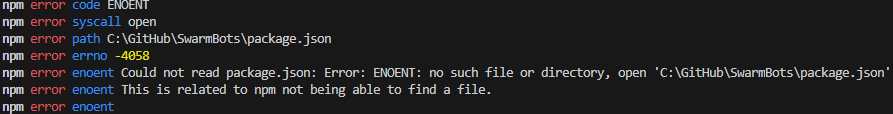
\includegraphics[width=0.8\textwidth, center]{img/GitHub_Buildprobleme.png}
  \caption{GitHub - Buildprobleme}
  \label{fig:GitHub_Buildprobleme}
\end{figure}
